\documentclass[a4paper,
               %boxit,        % check whether paper is inside correct margins
               %titlepage,    % separate title page
               %refpage       % separate references
               %biblatex,     % biblatex is used
               keeplastbox,   % flushend option: not to un-indent last line in References
               %nospread,     % flushend option: do not fill with whitespace to balance columns
               %hyphens,      % allow \url to hyphenate at "-" (hyphens)
               %xetex,        % use XeLaTeX to process the file
               %luatex,       % use LuaLaTeX to process the file
               ]{jacow}
%
% ONLY FOR \footnote in table/tabular
%
\usepackage{pdfpages,multirow,ragged2e} %
\usepackage{physics}% symbols frequent in physics with briefer commands
% CHANGE SEQUENCE OF GRAPHICS EXTENSION TO BE EMBEDDED
% ----------------------------------------------------
% test for XeTeX where the sequence is by default eps-> pdf, jpg, png, pdf, ...
%    and the JACoW template provides JACpic2v3.eps and JACpic2v3.jpg which
%    might generates errors, therefore PNG and JPG first
%
\makeatletter%
	\ifboolexpr{bool{xetex}}
	 {\renewcommand{\Gin@extensions}{.pdf,%
	                    .png,.jpg,.bmp,.pict,.tif,.psd,.mac,.sga,.tga,.gif,%
	                    .eps,.ps,%
	                    }}{}
\makeatother

% CHECK FOR XeTeX/LuaTeX BEFORE DEFINING AN INPUT ENCODING
% --------------------------------------------------------
%   utf8  is default for XeTeX/LuaTeX
%   utf8  in LaTeX only realises a small portion of codes
%
\ifboolexpr{bool{xetex} or bool{luatex}} % test for XeTeX/LuaTeX
 {}                                      % input encoding is utf8 by default
{\usepackage[utf8]{inputenc}}           % switch to utf8

\usepackage[USenglish]{babel}


%
% if BibLaTeX is used
%
% \ifboolexpr{bool{jacowbiblatex}}%
%  {%
% %   \addbibresource{refs.bib}
%   %\addbibresource{biblatex-examples.bib}
%  }{}
\listfiles

%%
%%   Lengths for the spaces in the title
%%   \setlength\titleblockstartskip{..}  %before title, default 3pt
%%   \setlength\titleblockmiddleskip{..} %between title + author, default 1em
%%   \setlength\titleblockendskip{..}    %afterauthor, default 1em

\begin{document}

\title{DRAFT: ONLINE OPTIMIZATION OF SIRIUS NONLINEAR OPTICS}

\author{M. M. S. Velloso\thanks{matheus.velloso@lnls.br}\textsuperscript{1}, F. H. de Sá, M. B. Alves, L. Liu\\ Brazilian Synchrotron Laboratory (LNLS), 13083-100, Campinas, Brazil \\
		X. Huang, SLAC National Accelerator Laboratory, [Postal Code] City, Country \\
		\textsuperscript{1}also at Gleb Wataghin Institute of Physics, University of Campinas, 13083-859, Campinas, Brazil 
}
	
\maketitle
%
\begin{abstract}
SIRIUS is the 4th generation storage ring-based synchrotron light source built and operated by the Brazilian Synchrotron Light Laboratory (LNLS). Beam accumulation at SIRIUS storage ring occurs in an off-axis scheme, using a nonlinear kicker (NLK), for which the efficiency depends on a sufficiently large dynamic aperture (DA). During the commissioning phase, the lattice configurations found by optimization of the model's DA and energy acceptance were implemented and rendered the machine an average injection efficiency of 85\%,  below the 95\% target for operating in the top-up mode. DA measurements also indicated a smaller aperture than predicted by the model, signalling the necessity of further optimization of the machine. This work presents the results of online optimization of SIRIUS nonlinear dynamics with the aim of increasing the machine's dynamic aperture and injection efficiency without compromising the off-momentum acceptance and Touschek lifetime. 
\end{abstract}


\section{INTRODUCTION}
At SIRIUS storage ring, the incoming beam is delivered at $x=-8.4~\unit{mm}$ where it is kicked by the NLK and captured into the ring acceptance. During the design phase, tracking simulations for this setup predicted a 99\% injection efficiency, considering a horizontal dynamic aperture of $-9~\unit{mm}$ in the horizontal plane \cite{Liu:IPAC2016-THPMR011}. This aperture was estimated from the model with the optimized nonlinear lattice configurations and realistic errors \cite{deSá:IPAC2016-THPMR012}. This same lattice was implemented in the machine during commissioning and currently renders an injection efficiency of about 85\% with corrected linear optics and coupling. With plans for SIRIUS storage ring to operate in top-up injection mode starting April 2023 (? not sure), it became imperative to improve the DA to achieve a high and reliable injection efficiency of a least $95\%$. 

Following recent experiences in other synchrotron facilities \cite{Huang:2015, Liuzzo:IPAC2016-THPMR015, Olsson:IPAC2018-WEPAL047, yang:ipac2022-tupopt064} online optimization was applied on the storage ring nonlinear lattice to mitigate the discrepancies between the model and the machine nonlinear dynamics performances. The experiments were carried using the Robust Conjugate Direction Search (RCDS) algorithm \cite{Huang:2013}, with the injection efficiency as objective function to be maximized upon changes in SIRIUS sextupole families strengths. The lattice was optimized in the nominal operation point with tunes $(49.08, 14.14)$, as well as in a new operation point of $(49.20, 14.25)$, which shall be referred to as Operation Points 1 and 2, respectively. Operation point 2 has drawn attention since recent measurements indicated it can mitigate the effects of orbit perturbations, reducing by half the integrated power spectrum of the beam post the $60~\unit{Hz}$ frequency.   

\section{SIRIUS NONLINEAR LATTICE}
 SIRIUS storage ring consists on a 20-cell five-bend-achromat (5BA) lattice with natural emittance of $0.25~\si{nm rad}$ at $3~\unit{GeV}$. The 5BA lattice design comprises a 5-fold symmetric configuration with alternating high and low horizontal betatron functions. A superperiod is composed of one high-beta and 3 low beta sections: A-B-P-B. The B and P low-beta sections are identical as far as first order optics is concerned; they differ in second order optics, i.e., the sextupoles are different. There 6 achromatic sextupole families and 15 chromatic families. Figure \ref{fig:sirius} shows the lattice periods. (keep figure? anything relevant info missing?)
  \begin{figure}[!h]
     \centering
     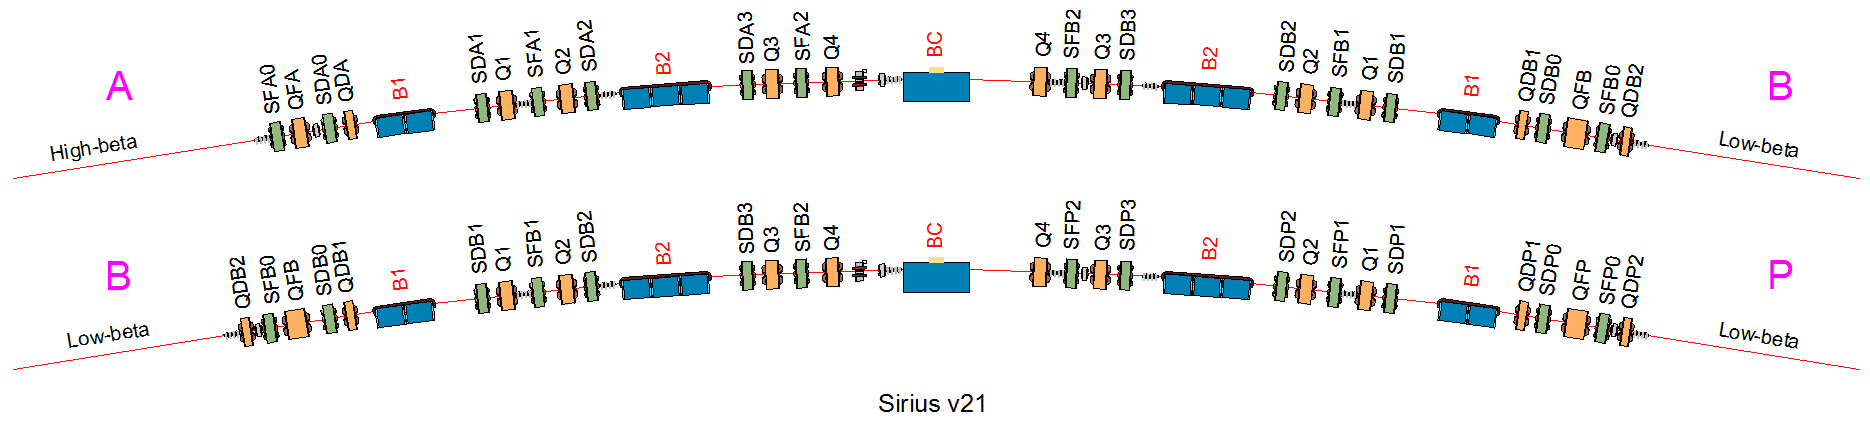
\includegraphics[width=\columnwidth]{SI_superperiod.png}
     \caption{SIRIUS 5BA Periods}
     \label{fig:sirius}
 \end{figure}
\section{OPTIMIZATION EXPERIMENTS}
\begin{figure*}[!h]
    \centering
    \includegraphics*[width=\textwidth]{oldtunes_runs123.pdf}
    \caption{Objective function (avg. injection efficiency of 5 pulses) history for RCDS optimization runs.}
    \label{fig:oldtunes_runs123}
\end{figure*}
\subsection{Optimization in the  operation point 1}
The objective function consisted on the average injection efficiency of five injection pulses with a noise-sigma of $\sigma \approx 1\%$. Since the current injection efficiency of $85\%$ is already quite high, the injection conditions were worsened for optimization by injecting the beam with a horizontal offset sufficient for efficiency to drop to $30$-$40\%$. SIRIUS injection dipole kicker for on-axis injection was used instead of the NLK since the NLK nonlinear field profile could be more sensitive to small factors during injection other than the DA. 

The optimization knobs consisted on the 6 achromatic sextupole families and a linear combination of the chromatic families. Families X plus Y and Z  (check which) tied together resulted in a 9-dimensional chromatic space. The 7-dimensional null-space of the chromaticity response matrix with with respect to the 9 knobs was calculated using the SIRIUS model. In total, the resulting parameter space consisted on 13 knobs. Families SFP1 and SFB1 were not included as knobs since they operate close to their upper limit.

With this setup, three optimization runs were performed. In run 1, RCDS optimized the efficiency from $\sim 40\%$ to $\sim 80\%$. Starting from the best configuration found in run 1, injection efficiency was worsened by further increasing the horizontal offset and another optimization run was fired. The same procedure was repeated for run 3., with the difference that the machine was cycled prior to loading the best solution. The objective function evaluations history for each run is shown in Figure~\ref{fig:oldtunes_runs123}.

\begin{figure}[!h]
   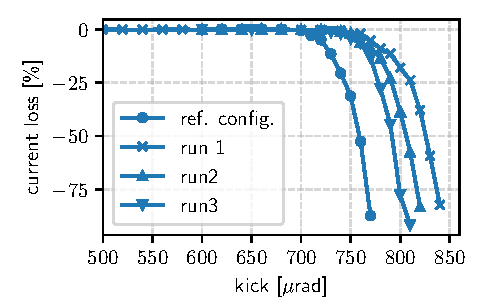
\includegraphics[width=\columnwidth]{old_tunes_kick_resilience.pdf}
   \caption{Current losses vs. horizontal dipole kick for the ref. config. and for the RCDS solutions. Losses in the ref. config. reach 50\% at $760~\si{\micro rad}$, while at run 1 config. the same loss is reached at $\sim 830~\si{\micro rad}$.}
   \label{fig:loss_kicks}
\end{figure}
For each one of best configurations found during runs 1, 2 and 3, turn-by-turn (TbT) data at increasing horizontal dipolar kicks was acquired. The DCCT current monitor allowed the determination of current loss as a function of the horizontal kick, which is shown in Figure~\ref{fig:loss_kicks}. TbT data also allowed for the reconstruction of the $(x,x^\prime)$ phase space. The BPM data for each turn is fitted using the machine model and allows the calculation of the corresponding angles $x^\prime$. Figure~\ref{fig:oldtunes_phase} shows the reconstructed phase spaces for the reference configuration (ref. config) and the best configurations found during run 1, 2, and 3 at the smallest kick for which the current loss is larger than $50\%$. These figures allow for the comparison of areas, which is presented in Figure~\ref{fig:oldtunes_areas}.
\begin{figure}[!h]
    \centering
    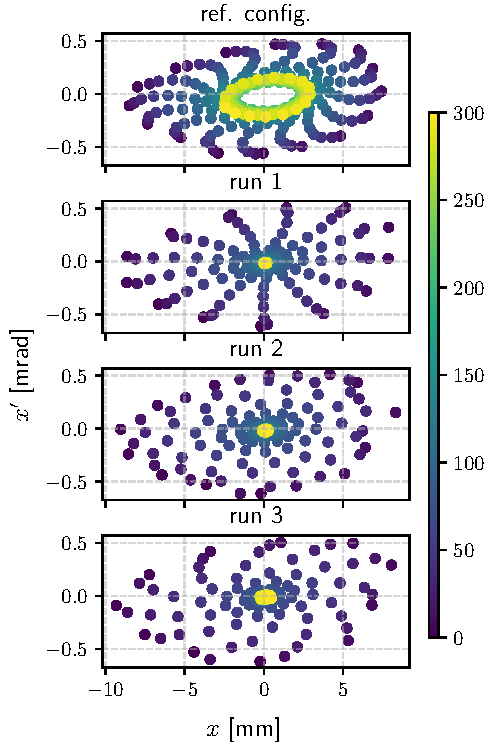
\includegraphics[width=\columnwidth]{old_tunes_phase.pdf}
    \caption{Phase portraits reconstruction by fitting TbT data collected for each configuration at kicks providing loss rates of $\geq 50\%$. Color code indicates the turns. Horizontal dipole kicks for ref. config: $760~\unit{\micro rad}$, run 1: $820~\unit{\micro rad}$, run 2: $810~\unit{\micro rad}$, run 3: $800~\unit{\micro rad}$.}
    \label{fig:oldtunes_phase}
\end{figure}
\begin{figure}[!h]
   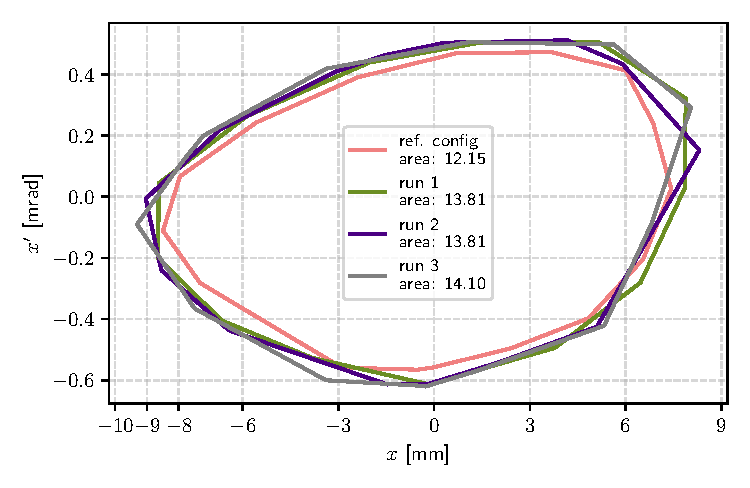
\includegraphics[width=\columnwidth]{phase_areas.pdf}
   \caption{Phase-space area comparison for each reconstructed phase-portrait of Fig.~\ref{fig:oldtunes_phase}. Areas in $\unit{mm}~\unit{mrad}$.}
   \label{fig:oldtunes_areas}
\end{figure}

\begin{table}[!h]
\centering
\caption{Injection efficiencies and horizontal dynamic aperture for the ref. config. and the best RCDS solutions (check archiver to get statistics)} 
\begin{tabular}{ccc}
\hline
configuration & \begin{tabular}[c]{@{}c@{}}injection efficiency\\ $[\%]$\end{tabular} & \begin{tabular}[c]{@{}c@{}}$x_{\text{min}}$\\ $[\unit {mm}]$\end{tabular} \\ \hline
ref-config    & $85\pm?$                                                              & $-8.50$                                                           \\
run 1         & $92\pm$                                                               & $-8.65$                                                           \\
run 2         & $99\pm$                                                               & $-9.04$                                                           \\
run 3         & $89\pm$                                                               & $-9.31$                                                           \\ \hline
\end{tabular}
\label{table1}
\end{table}
Table~\ref{table1} shows the injection efficiency achieved for each configuration in off-axis NLK injection. It also shows the minimum horizontal offsets reached in the TbT data of Figures~\ref{fig:oldtunes_phase} and~\ref{fig:oldtunes_phase}. Interestingly, neither the configuration with the largest kick resilience, run 1, nor the configuration with the largest phase-space area are the ones rendering the best injection efficiency (run 2). This differs from the experience in other accelerators, in which there is a more direct equivalence between optimizing kick resilience (minimizing beam loss at increasing kicks) and the injection efficiency and DA area increase (review others work and check this statement). Lifetime at $60~\unit{mA}$ was measured for run 2 best configuration and differed from the ref. config. by an hour ($21~\unit{hr}$ for ref. config. vs $20~\unit{hr}$ for run 2). There was also a small chromaticity drift from $(2.33, 2.53)$ in ref. config. to $(2.24, 2.3)$ in run 2 best solution.  

\subsection{Optimization in the operation point 2}
 The non-optimized machine at opteration point 2 had injection efficiency of $56\%$. Two optimization runs were carried out. In run 1, the same knobs used in the previous three runs were used. In run 2, the SDP1 and SFP1 families had their strengths lowered and were included as knobs. The chromatic set of knobs consisted in X, Y, X (check this). The 6 achromatic families plus 11 (check this) knobs spanning the null-space of the chromaticity response matrix constituted the 17 knobs used during run 2. Objective function evaluation history is shown in Figure~\ref{fig:newtunes_runs12}. Run 1 actually consisted on 4 runs, while run 2 consists on 3. Each significant drop in efficiency represents interrupting the optimization, loading the best solution at the time, worsening injection conditions by increasing the offset, and continuing the optimization routine.
\begin{figure}[!h]
   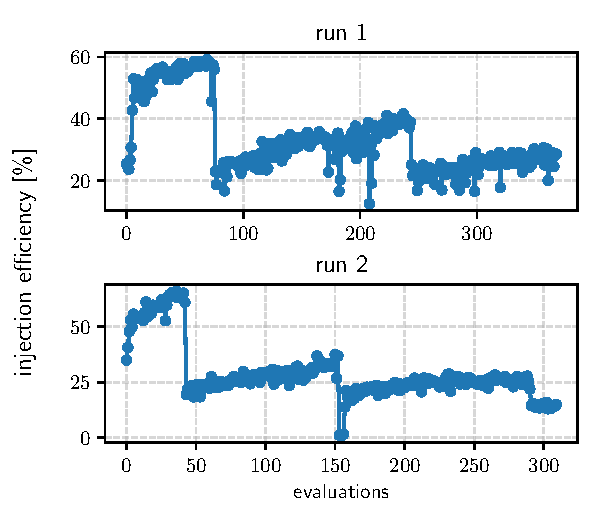
\includegraphics[width=\columnwidth]{newtunes_runs12.pdf}
   \caption{Objective function (avg. injection efficiency of 5 pulses) history for RCDS optimization runs in operation point 2.}
   \label{fig:newtunes_runs12}
\end{figure}

TbT data at increasing horizontal dipolar kicks for each configuration was acquired and allowed the determination of current losses vs. kicks, Fig.~\ref{fig:loss_kicks_newtunes}, and also the reconstruction of phase space at the kicks yielding current losses larger than $50\%$, Fig~\ref{fig:newtunes_phase}. Figure~\ref{fig:newtunes_phase_areas} compares the phase space areas for the non-optimized configuration as well as the configurations found during runs 1 and 2 in the new operation point. Table~\ref{table2} compiles the results for the configurations in the new tunes: best off-axis injection efficiencies and largest horizontal displacements reached at current loss larger than $50\%$. The configuration found during run 1 yielded the best injection efficiency, the largest phase-space area, largest kick resilience and also larger lifetime than the non-optimized configuration ($21~\unit{hrs}$, run 1 vs $18~\unit{hrs}$, non-optimized, $60~\unit{mA}$). 
\begin{figure}[!h]
   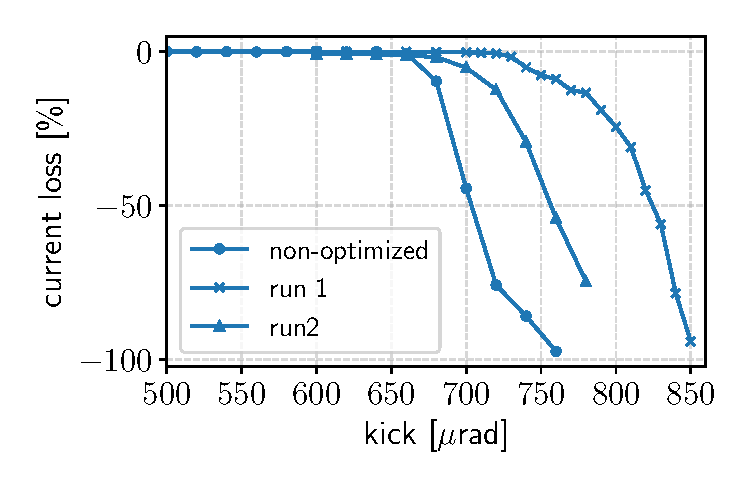
\includegraphics[width=\columnwidth]{new_tunes_kick_resilience.pdf}
   \caption{Current losses vs. horizontal dipole kick for the non-optimized configuration at operation point 2 and for the RCDS solutions. Losses in the non-optimized config. reach 50\% at $\sim710~\si{\micro rad}$, while at run 1 config. the same loss is reached at $\sim 830~\si{\micro rad}$.}
   \label{fig:loss_kicks_newtunes}
\end{figure}

\begin{figure}
   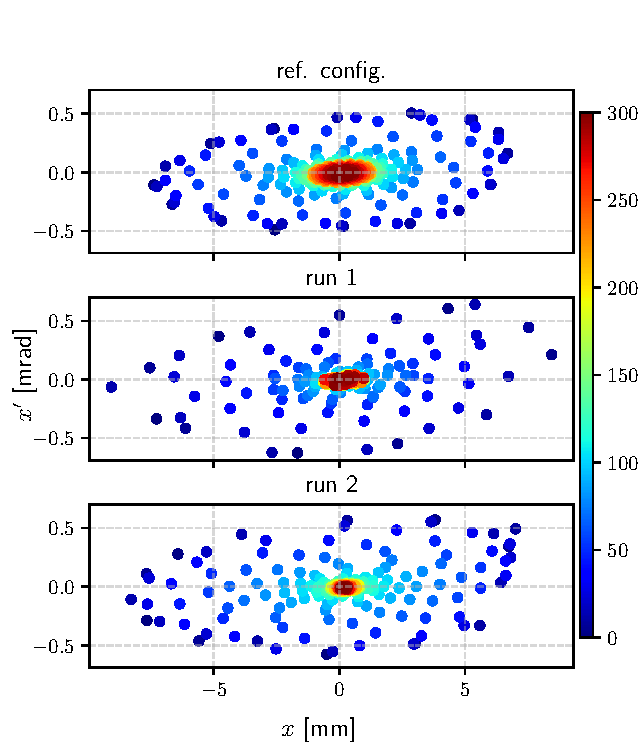
\includegraphics[width=\columnwidth]{new_tunes_phase.pdf}
   \caption{Phase portraits reconstruction by fitting of TbT data collected for each configuration at kicks providing loss rates of $\geq 50\%$ in operation point 2. Color code indicates the turns. Horizontal dipole kicks for non-optimized: $~\unit{\micro rad}$, run 1: $~\unit{\micro rad}$, run 2: $~\unit{\micro rad}$. Correct ref. config to non-optimized. Correct colormap to viridis.}
   \label{fig:newtunes_phase}
\end{figure}

\begin{figure}
   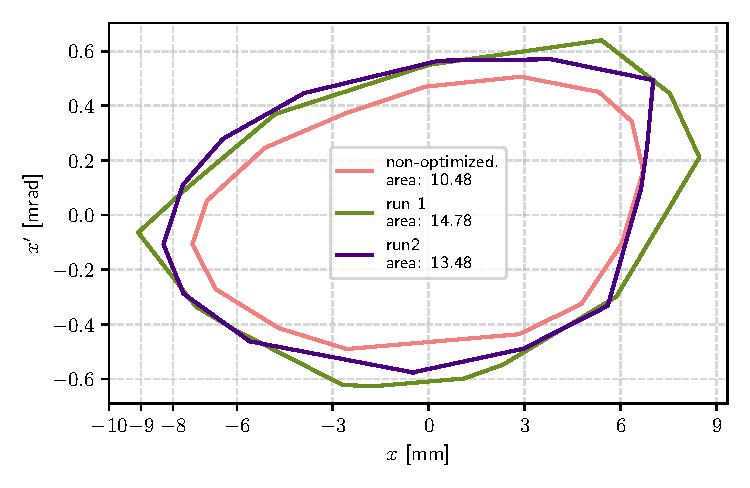
\includegraphics[width=\columnwidth]{new_tunes_phase_areas.pdf}
   \caption{Phase space area comparison for each reconstructed phase-portrait of Fig.~\ref{fig:newtunes_phase}. Areas in $\unit{mm}~\unit{mrad}$.}
   \label{fig:newtunes_phase_areas}
\end{figure}



\begin{table}[]
\centering
\caption{Main parameters for the non-optimized and optimized configs. in the new tunes}
\begin{tabular}{ccc}
\hline
configuration & \begin{tabular}[c]{@{}c@{}}injection efficiency\\ $[\%]$\end{tabular} & \begin{tabular}[c]{@{}c@{}}$x_{\text{min}}$\\ $[\unit {mm}]$\end{tabular} \\ \hline
non-optimized & $--$                                                                  & $-7.39$                                                            \\
run 1         & $82\pm$                                                               & $-9.08$                                                            \\
run 2         & $--\pm$                                                               & $-8.29$                                                            \\ \hline
\end{tabular}
\label{table2}
\end{table}


\section{CONCLUSIONS}
Mention more recent attempts at the newest newtunes?
%
% only for "biblatex"
%
% \ifboolexpr{bool{jacowbiblatex}}%
% 	{\printbibliography}%
% 	{%
	% "biblatex" is not used, go the "manual" way
	
	%\begin{thebibliography}{99}   % Use for  10-99  references
	\begin{thebibliography}{9} % Use for 1-9 references
	
        
%     \bibitem{Alves:IPAC21-MOPAB260}
%        M. B. Alves,
%        \textquotedblleft{Optics Corrections with LOCO on Sirius Storage Ring}\textquotedblright,
%        in \emph{Proc. IPAC’21}, Campinas, Brazil, May 2021, pp. 825--828.
%        \url{doi:10.18429/JACoW-IPAC2021-MOPAB260} 

    \bibitem{Liu:IPAC2016-THPMR011}
        L. Liu, X.R. Resende, A.R.D. Rodrigues, F. H. de Sá,
       \textquotedblleft{{I}njection {D}ynamics for {S}irius {U}sing a {N}onlinear {K}icker}\textquotedblright,
       in \emph{Proc. IPAC’16}, Busan, Korea, May 2016, pp. 3406--3408.
       \url{doi:10.18429/JACoW-IPAC2016-THPMR011} 
 
    \bibitem{deSá:IPAC2016-THPMR012}
        F. H. de Sá, L. Liu, X.R. Resende,
       \textquotedblleft{{O}ptimization of {N}onlinear {D}ynamics for {S}irius}\textquotedblright,
       in \emph{Proc. IPAC’16}, Busan, Korea, May 2016, pp. 3409--3412.
       \url{doi:10.18429/JACoW-IPAC2016-THPMR012}       
       
	\bibitem{Huang:2013}
		X. Huang, J. Corbett, J. Safranek, J. Wu,
		\textquotedblleft{An algorithm for online optimization of accelerators}\textquotedblright,
		\emph{Nucl.  Instr. Meth.}, vol 726, pp. 77--83, 2013.
        \url{https://doi.org/10.1016/j.nima.2013.05.046} 

    \bibitem{Huang:2015}
		X. Huang, J. Safranek,
		\textquotedblleft{Online optimization of storage ring nonlinear beam dynamics}\textquotedblright,
		\emph{Phys. Rev. ST Accel. Beams}, vol 18, p. 18, .
        \url{10.1103/PhysRevSTAB.18.084001} 
 
    \bibitem{Liuzzo:IPAC2016-THPMR015}
        S.M. Liuzzo, \emph{et al.},
        \textquotedblleft{RCDS Optimizations for the ESRF Storage Ring}\textquotedblright,
        in \emph{Proc. IPAC’16}, Busan, Korea, May 2016, pp. 3420--3423.
       \url{doi:10.18429/JACoW-IPAC2016-THPMR015}   
    
    \bibitem{Olsson:IPAC2018-WEPAL047}
       D.K. Olsson,
       \textquotedblleft{Online Optimisation of the MAX IV 3 GeV Ring Dynamic Aperture}\textquotedblright,
    % --- abbreviated form (published paper) - JACoW template Feb 2018 ---
       in \emph{Proc. IPAC'18}, Vancouver, BC, Canada, Apr. 4,, pp. 2281--2283,
       \url{doi:10.18429/JACoW-IPAC2018-WEPAL047}
    % --- complete form (published paper) - JACoW template Feb 2018 ---
    %  in \emph{Proc. 9th International Particle Accelerator Conference (IPAC'18)}, Vancouver, BC, Canada, Apr. 4,,
    %  pp. 2281--2283, \url{doi:10.18429/JACoW-IPAC2018-WEPAL047}
    % --- additional material ---
    %  ISBN: 978-3-95450-184-7, \url{http://jacow.org/ipac2018/papers/wepal047.pdf}
    
    \bibitem{yang:ipac2022-tupopt064}
        X. Yang,\emph{et al.},
       \textquotedblleft{Online Optimization of NSLS-II Dynamic Aperture and Injection Transient}\textquotedblright,
        in \emph{Proc. IPAC'22}, Bangkok, Thailand, Jun. 2022, pp. 1159--1162.
    % --- complete form (published paper) - JACoW template Feb 2018 ---
    %  in \emph{Proc. 13th International Particle Accelerator Conference (IPAC'22)}, Bangkok, Thailand, Jun. 2022, pp. 1159--1162.
       \url{doi:10.18429/JACoW-IPAC2022-TUPOPT064}
    
   
	\end{thebibliography}

% } % end \ifboolexpr
%
% for use as JACoW template the inclusion of the ANNEX parts have been commented out
% to generate the complete documentation please remove the "%" of the next two commands
% 
%\newpage

%\include{annexes-A4}

\end{document}
